\chapter{Характеристика та аналіз предметної галузі} 
\label{chap:first}

\section{Характеристика предметної області та об’єкта дослідженняі}

Мова DDlog є сучасним діалектом мови Datalog.

Мова Datalog була створеня для зручної роботи з логічними моделями. Проте ряд істотних недоліків залишив цю мову в стані академічного інструменту для дослідників. Цими недоліками були:
\begin{itemize}

\item Відстуність системи типів, що істотно підвищувало складність і створення і відладки програм

\item В оригінальній версії мова Datalog не мала ніяких способів виконувати процедури, тому навіть прості на перший погляд логічні конструкції могли мати дуже нетривіальні реалізації.

\item В більшості реалізацій моделі виконувалися інтрепретаторами, це призводило до зниження ефективності роботи, що в кінці робило неможливим використання тих систем навіть на масштабі локальних БД (SQLite).

\end{itemize}

Разом з тим, було розвинено реляційну модель та створено перші реляційні СКБД, цей прорив витіснив мову Datalog з індустрії на багато років. Реляційна модель є виразною  через конструкціїї логічні конструкції мови Datalog, тому є підмножиною логічної мови. З часом були виявлені недоліки реляційних моделей що призвело до виникнення парадігми NewSQL, та звернули погляди фахівців і науковців назад до мови Datalog.

\section{Дослідження існуючих інформаційних систем для обраної предметної області}

Існує багато програмних засобів для роботи за мовою Datalog та її розширеннями. Datalog в його багато численних реалізаціях зазвичай не має системи типів, а якщо і має то зазвичай базову, без можливості декларації своїх типів даних.

Проте, я хотів би звернути увагу на декілька з них:

\begin{enumerate}

\item Flix\cite{flix} -  мова програмування що реалізує можливості логічного програмування через вбудовану підмову - діалект Datalog. Одночасно плюсом та мінусом є те, що це повноцінна мова програмування, з цього випливає те, що не існує легкого способу експортувати моделі як компоненти, проте завдяки цьому можливо швидке прототипування логічних моделей.

\item Souffle\cite{souffle}. Основне призначення - створення проміжних програмних компонентів для використання в компільованих программах. Теж діалект Datalog. Плюсом є те, що результатом використання є оптимізований C++ код, яккий можна застосовувати як завгодно.

\item DDLog\cite{ddlog}. Основне призначення - створення проміжних інкрементальних програмних компонентів для використання в компільованих программах. Мова DDlog має можливість вираховувати зміни в вихідних фактах при внесенні змін в вхідні факти. Це дозволяє побудувати реактивну логічну модель з її декларатовного опису. Ця система генерує модулі мови Rust, що передбачують роботу в розподіленному середовищі.

\end{enumerate}

Табличне порівняння: 

\begin{flushright}\small {Таблиця 1.1} \end{flushright}
\begin{center}
Порівняння існуючих систем
\small{
\begin{tabular}{ | c | c | c |  }
\hline
 Назва & Сценарій використання (основний)  & Інкрементальність \\ 
\hline
 Flix & Мова програмування & Не має \\  
\hline
 Souffle & Програмні компоненти & Не має \\  
\hline
 DDLog & Програмні компоненти & Є \\  
\hline
\end{tabular}
}
\end{center}

З приведеного вище порівняння, можна сказати що нині, чистих та сучасних Datalog систем орієнтованих на неопосередковану роботу з логічними моделями Datalog не існує.

\newpage

\section{Розробка концепції інформаційної системи}

В запропонованій системі <<Play DDlog>> використовується діалект Datalog DDlog.  В якості інтерфейсу користувача обрано веб інтрефейс тому що він гарантує максимальну доступність результуючого додатку.

Скетч інтерфейсу користувача наведено на рис. 1.1

\begin{center}
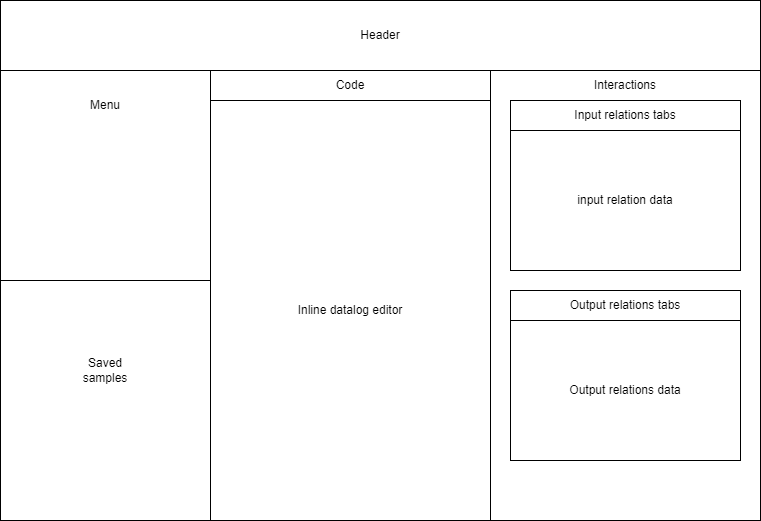
\includegraphics[width=8cm]{first_ui_sketch}

Рисунок 1.1 -- Скетч інтерфейсу користувача

\end{center}